\chapter{Working with Resource Components}
Resource Components are ICE Components which contain a grid of visualization
resources. These resources can display files from a variety of sources,
such as CSV files or VisIt visualizations. Geometry and Mesh editors allow for
editing of shapes or meshes. All three can be added to an Item to offer
visualization of data.

\section{Prerequisites}

This tutorial assumes you will be making use of the sample classes in the
org.eclipse.ice.demo.visualization package for convenience. The two relevant
classes are VisualizationModel and VisualizationModelComplete. The former is an
example of a bare bones ICE Item, while the latter is the same class with all
the extra code required for the visualization components already added in.

If you are writing your own extension of ICE's Item class, then the same
principles can be used to add these components to it. See the New Item
Generation Tutorial, in the docs/newItemGeneration/ folder of the ICE repo for
details on how to create an Item.

You will also need access to an installation of VisIt version $2.9.2$. If
not already installed, there is a copy of the software in the VisIt folder of
your USB drive. Windows users should open the Windows installer, while users of
other OSs can just copy the appropriate folder onto their machine.

\section{Adding the Components}

First, open the Item file by double clicking it in the \texttt{Package
Explorer}. For the tutorial, this will be VisualizationModel.java in the
org.eclipse.ice.demo. visualization.model package. Its location can be seen in
figure \ref{fig:demostructure}.

\begin{figure}[!H]
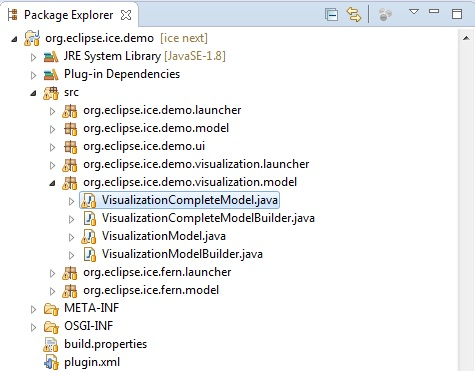
\includegraphics[width=\textwidth]{images/DemoPackageStructure}
\centering
\caption{The package structure for org.eclipe.ice.demo bundle}
\label{fig:demostructure}
\end{figure}

First, add the neccesary imports for the components being added to your Item. 

\begin{verbatim}
import java.io.IOException;
import org.eclipse.core.resources.IFile;
import org.eclipse.core.resources.ResourcesPlugin;
import org.eclipse.eavp.viz.modeling.ShapeController;
import org.eclipse.eavp.viz.modeling.ShapeMesh;
import org.eclipse.eavp.viz.modeling.base.BasicView;
import org.eclipse.ice.datastructures.form.GeometryComponent;
import org.eclipse.ice.datastructures.form.MeshComponent;
import org.eclipse.ice.datastructures.form.ResourceComponent;
import org.eclipse.ice.datastructures.resource.VizResource;
\end{verbatim}

Next, copy and paste the following example code into the end of your Item's
setupForm() method.

\begin{verbatim}
//Create the resource component
ResourceComponent resourceComponent = new ResourceComponent();

//Set the component's data members
resourceComponent.setName("Resources");
resourceComponent.setDescription("Results");
resourceComponent.setId(2);

//Declare the files and resources
VizResource csvResource = null;
VizResource visItResource = null;
IFile csvFile = null;
IFile visItFile = null;


//If the file was found, create the CSV resource and add it to the component
try{
			
	//Open the files
	csvFile = ResourcesPlugin.getWorkspace().getRoot().getProject("itemDB")
		.getFile("fib8.csv");
	visItFile = ResourcesPlugin.getWorkspace().getRoot().getProject("itemDB")
		.getFile("tire.silo");
			
	//If the file was found, create the CSV resource and add it to the component.
	if(csvFile.exists()){
		csvResource = new 
                    VizResource(csvFile.getLocation()
                    .toFile());
    	resourceComponent.addResource(csvResource);
	}
				        
	//If the file was found, create the VisIt resource and add it to 
	//the component
	if(visItFile.exists()){
		visItResource = new 
                    VizResource(visItFile.getLocation()
                    .toFile());
		resourceComponent.addResource(visItResource);
	}
}
catch(IOException e){
	e.printStackTrace();
}

//Create the geometry component
ShapeController geometryRoot = new ShapeController(new
    ShapeMesh(), new BasicView());
GeometryComponent geometryComponent = new 
    GeometryComponent();
geometryComponent.setGeometry(geometryRoot);

//Create mesh component
MeshComponent meshComponent = new MeshComponent();

//Add the components to the form
form.addComponent(resourceComponent);
form.addComponent(geometryComponent);
form.addComponent(meshComponent);	
		
//Set the context on the Form
form.setContext("visualization");
\end{verbatim} 

This code will add a Resource Component, Geometry Component, and Mesh Component
to your Item and load fib8.csv and tire.silo into the Resource Component.

You will also need to add the org.eclipse.ice.demo bundle to your operating
system's run configuration, as explained in the new item generation tutorial
(found in docs/newItemGeneration in the ICE repo). 

You can compare your code to the VisualizationCompleteModel.java file, which has
a working version of the Item with the tutorial code put in. 

When done, launch ICE. If you have never launched ICE before, go to the
org.eclipse.ice.product bundle, right click the .launch file for your operating
system, and select the first option under the \texttt{Run as\ldots} submenu.

\section{Using the Resource Component}

ICE uses an instance of VisIt, a visualization code from Lawrence Livermore
National Laboratory, running in another process for visualization. ICE can also
use ParaView, but this tutorial will only cover VisIt, as the processes for
conencting to ParaView and using a ParaView Plot Editor are largely similiar to
those for VisIt.

\subsection{Establishing a VisIt Connection}

In order to visualize resources containing VisIt files, ICE must be connected to
a running VisIt installation. To set up this connection, select \texttt{Windows}
$\rightarrow$ \texttt{Preferences...} in ICE's menu bar. (On Mac OS X,
\texttt{Preferences} is instead located under \texttt{ICE} in the menu
bar.)

\begin{figure}[!h]
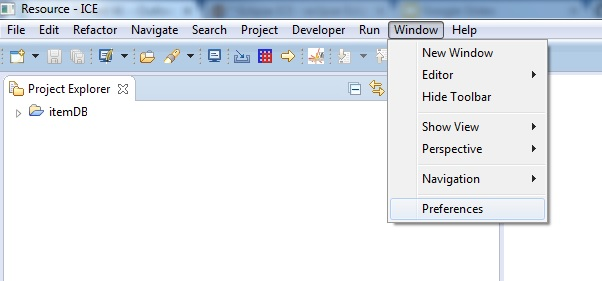
\includegraphics[width=12cm]{images/ICEPreferences}
\centering
\caption{The ICE \texttt{Preferences Menu} for Windows and Linux. It will be
located under \texttt{ICE} instead of \texttt{Window} on Mac.}
\label{fig:icepreferences}
\end{figure}


Select \texttt{Visualization} $\rightarrow$ \texttt{VisIt} in the tree on the
left side of the \texttt{Preferences} window.

\begin{figure}[!h]
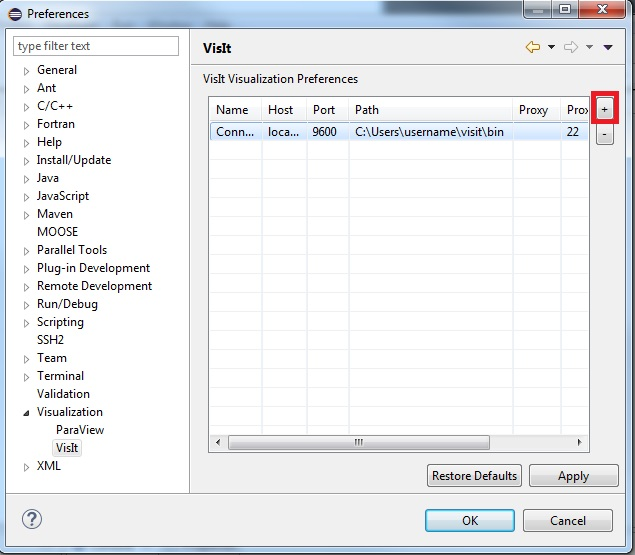
\includegraphics[width=12cm]{images/VisualizationPreferences}
\centering
\caption{The \texttt{VisIt} preferences page in the \texttt{Preferences}
dialog. The hilighted button will add a row for a new connection to the table.}
\label{fig:visualizationpreferences}
\end{figure}


Press the button with a "+" symbol in the upper right of the
\texttt{Preferences Menu} (highlighted in Figure
\ref{fig:visualizationpreferences}) to add a new row to the table.
Click on the \texttt{Path} cell of the new row and put the path of your installation of VisIt.

For example, on \texttt{Windows}, if assuming a username of "username", and
VisIt was installed in the default location, the path will be:

\texttt{C:\textbackslash Users\textbackslash
username\textbackslash AppData\textbackslash Local\textbackslash
Programs\textbackslash LLNL\textbackslash VisIt 2.9.2.}

On \texttt{Linux}, the path will be based on where you extracted the 
visit2\_9\_2.linux-x86 folder, ending with /visit2\_9\_2.linux-x86\_64/bin. If
you unzipped it to the desktop, it will be:
 
\texttt{/home/username/Desktop/visit2\_9\_2.linux-x86\_64/bin}

On \texttt{Mac OS}, the path will be based on the location you put the Visit
application. If placed in the Applications folder it will be

\texttt{/Applications}

Press \texttt{Apply}, then \texttt{OK}, both in the lower right hand corner of
the \texttt{Preferences Menu}.
ICE will now open and connect to this VisIt installation each time ICE is opened.

\subsection{Opening Your Item}
Before opening your new Item, select the itemDB folder in the \texttt{Project
Explorer} and press the import button, highlighted below.

\begin{figure}[!h]
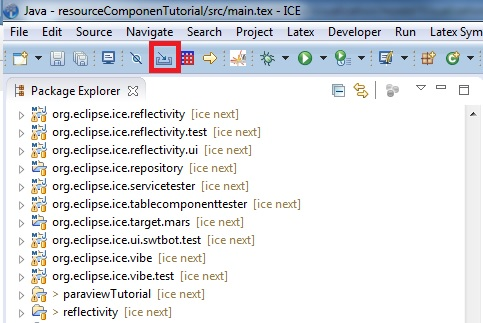
\includegraphics[width=12cm]{images/ImportButton}
\centering
\caption{ICE's \texttt{import} button.}
\label{fig:importbutton}
\end{figure}

Select the files you want to visualize and click OK. For the tutorial, these
should be the fib8.csv and tire.silo files from the USB drive's Data directory.
You should now see the two files within the itemDB folder.

Then select \texttt{New} $\rightarrow$ \texttt{Other\ldots} from the toolbar. In
the new dialog, select the \texttt{Create Item Wizard} and hit \texttt{Next}.
Then select \texttt{Visualization Model} and press \texttt{Finish}. You can also select the
\texttt{Visualization Model (Pre-completed)} if you skipped the first part of
the tutorial.

Finally, switch to the ICE Perspective to ensure that the neccesary Views will
be open. To do this, click the \texttt{Open Perspective} button in the upper right
of the workbench screen.

\begin{figure}[!h]
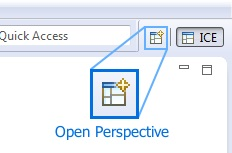
\includegraphics{images/ICE_OpenPerspective}
\centering
\caption{ICE's \texttt{Open Perspective} button.}
\label{fig:openpersepctive}
\end{figure}

In the dialog, select \texttt{ICE} and press {OK}.

\subsection{Managing the Resources}

Your Item should look like this when it loads.

\begin{figure}[!h]
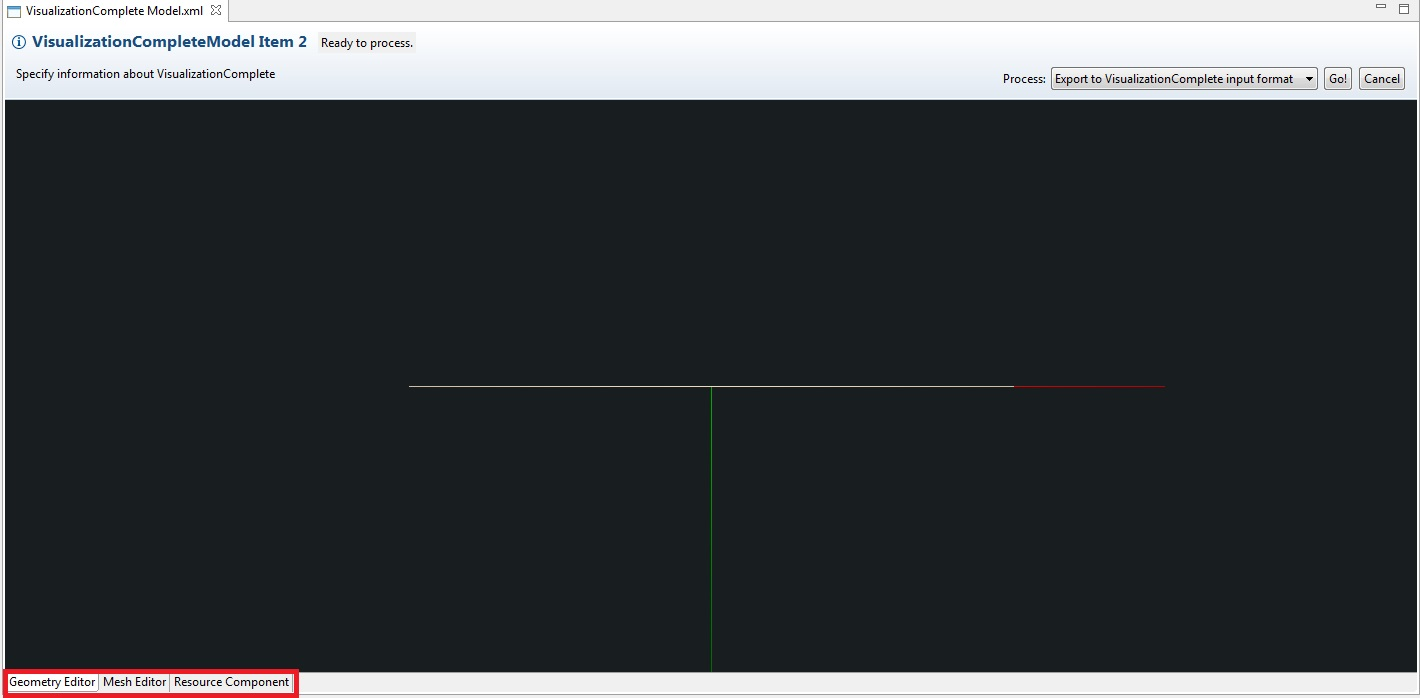
\includegraphics[width=12cm]{images/ItemTabs}
\centering
\caption{The \texttt{Visualization Model} after it is initially opened.
Hilighted in the lower left are the tabs for the three components, the
\texttt{Geometry Editor}, the \texttt{Mesh Editor}, and the \texttt{Resource
Component}.}
\label{fig:itemtabs}
\end{figure}

In the lower left of the \texttt{Visualization Model} are three tabs, hilighted
in Figure \ref{fig:itemtabs}.
Switch to the \texttt{Resource Component} tab in your Item and tothe \texttt{Resources} tab on the left, as shown below.

\begin{figure}[!h]
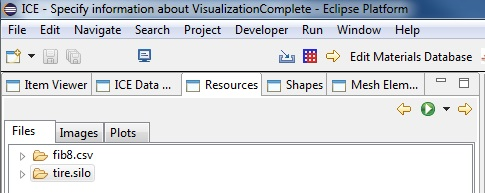
\includegraphics[width=12cm]{images/ResourcesTab}
\centering
\caption{The \texttt{ICE Perspective}'s \texttt{Resources} tab.}
\label{fig:resourcestab}
\end{figure}

Double click on both the file names to load them into the Resource Component.

At the top left of the \texttt{Visualization Model} will be controls for the
component's layout.

\begin{figure}[!h]
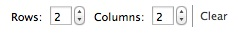
\includegraphics{images/ResourceComponentControls}
\centering
\caption{The layout controls for the \texttt{Resource Component}.}
\label{fig:resourcecomponentcontrols}
\end{figure}

The \texttt{Clear} button will close all plots in the component. The other two
controls will allow you to specify the number of rows and columns in the grid.
Be careful when reducing them, as any plots which no longer fit in the grid will
be closed.

If you hover over a plot, a button will appear in its upper left hand corner.
Clicking it will close that plot. 

\begin{figure}[!h]
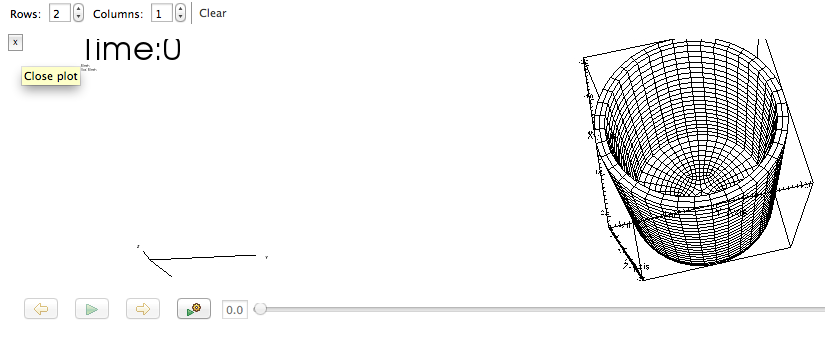
\includegraphics[width=12cm]{images/ClosePlotButton}
\centering
\caption{The X button in the upper left will close the plot.}
\label{fig:closeplotbutton}
\end{figure}

\subsection{Interacting with VisIt Plots}

\begin{figure}[!h]
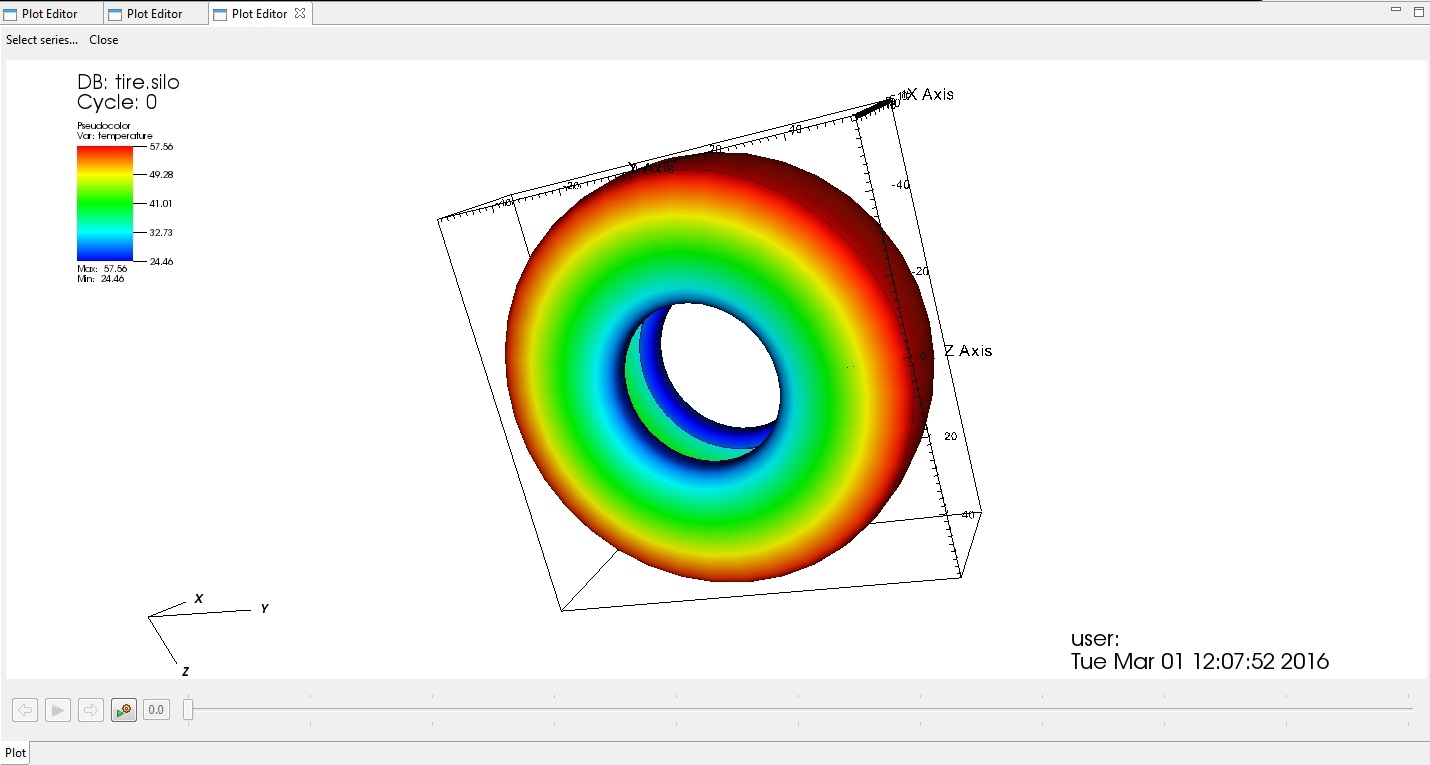
\includegraphics[width=12cm]{images/VisItPlot}
\centering
\caption{An example of a file open in VisIt displayed in a \texttt{Plot
Editor}.}
\label{fig:visitplot}
\end{figure}

A VisIt plot will contain a 3D visualization of some model. You can click and
drag within the plot to rotate the image and zoom by scrolling your mouse wheel.
Right clicking in the plot will open a context menu, providing options for how
the model will be displayed.

At the bottom of the plot will be a series of controls for animation. If your
plot does not have time series data, they will be greyed out. 

\begin{figure}[!h]
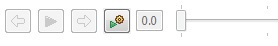
\includegraphics[width=12cm]{images/TimeSliderWidget} 
\centering
\caption{The \texttt{Plot Editor}'s animation controls.}
\label{fig:timesliderwidget}
\end{figure}

The plot can be set to display an arbitrary time step by either dragging the
slider or by typing a time into the box to its left.

\subsection{Interacting with CSV Plots}

\begin{figure}[!h]
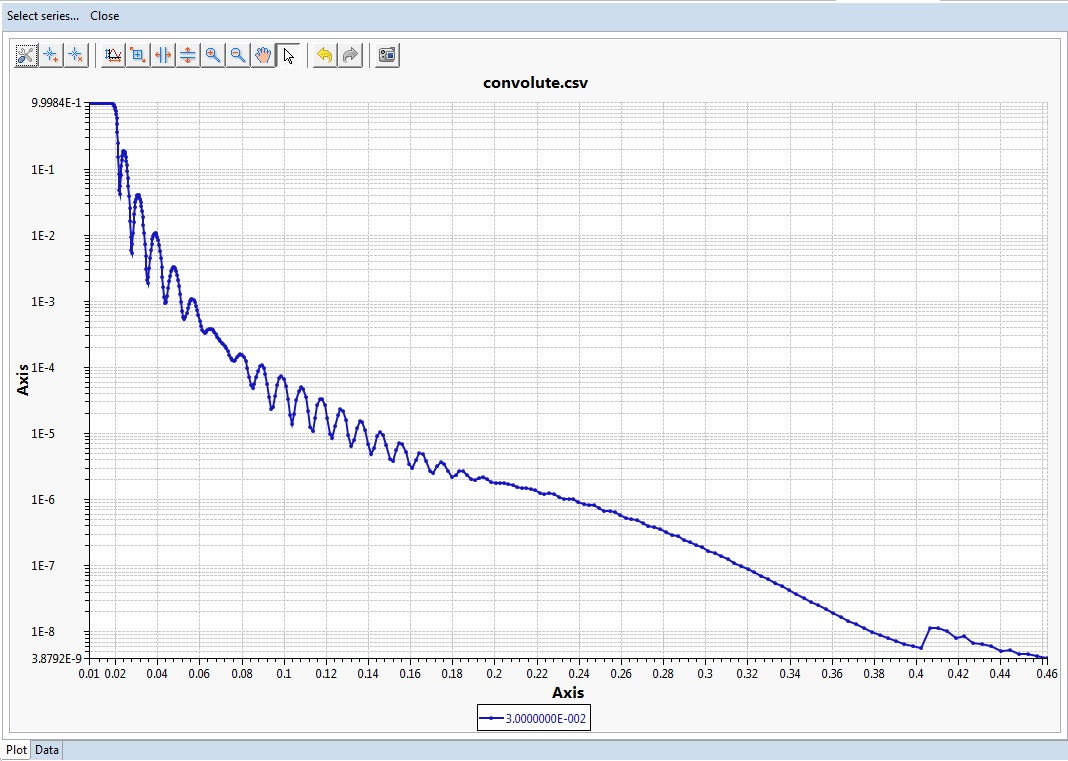
\includegraphics[width=12cm]{images/CSVGraph}
\centering
\caption{An example of a CSV file. The Y axis is displayed on a logarithmic
scale.}
\label{fig:CSVGraph}
\end{figure}

The top of the CSV plot has a row of buttons which control various aspects of
the graph's presentation. Right clicking will open a context menu allowing you
to choose which of the available series to plot.

\subsection{Editing 3D Structures}

ICE also contains capabilities to render graphics with the Geometry Editor and
Mesh Editor. Programatically populating these editors with custom input is
beyond the scope of this tutorial. However, what follows will be a brief
overview of the editors' functionality.

\subsubsection{The Geometry Editor}

Now switch to the \texttt{Geometry Editor} tab in you the \texttt{Visualization
Model} and the \texttt{Shapes} tab on the left.

Clicking the \texttt{Add Primitives} button will display a drop down of
primitive shapes which can be added to the scene.

\begin{figure}[!h]
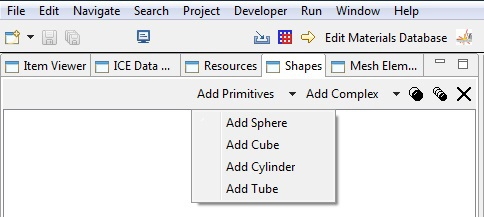
\includegraphics[width=12cm]{images/AddPrimitiveShape}
\centering
\caption{The \texttt{Add Primitives} button displays a menu of shapes to add.}
\label{fig:addprimitiveshape}
\end{figure}

Complex shapes can similarly be added using the \texttt{Add Complex} button.

\begin{figure}[!h]
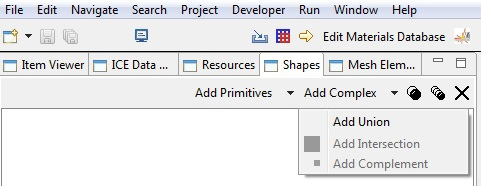
\includegraphics[width=12cm]{images/AddComplexShape}
\centering
\caption{The \texttt{Add Complex} button can add a Union of shapes.}
\label{fig:addcomplexshape}
\end{figure}

Primitive shapes can be added under complex shapes by selecting anything beneath
the desired parent complex shape before adding the new primitive.

\begin{figure}[!h]
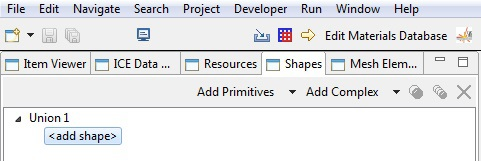
\includegraphics[width=12cm]{images/ComplexShapeTree}
\centering
\caption{An example of a constructive solid geometry tree in the
\texttt{Shapes} tab. Adding shapes with the highlighted leaf selected will
cause them to become children of Union 1.}
\label{fig:complexshapetree}
\end{figure}

The three other buttons are responsible for creating copies of or removing
selected shapes from the tree. 

The Transformation View, in the lower left of the workbench screen, has spaces
to set the rotation, scale, and translation of a selected object.

\begin{figure}[!h]
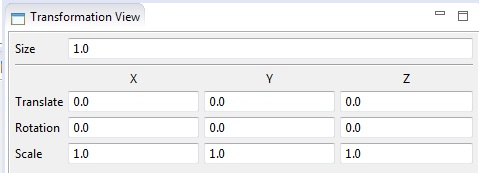
\includegraphics[width=12cm]{images/TransformationView}
\centering
\caption{The \texttt{Transformation View}.}
\label{fig:transformationview}
\end{figure}

\subsubsection{The Mesh Editor}

Now switch to the \texttt{Mesh Editor} tab in your Item and \texttt{Mesh
Elements} tab on your left.

Clicking within the grid will create a vertex, until the fourth completes the
polygon.

\begin{figure}[!h]
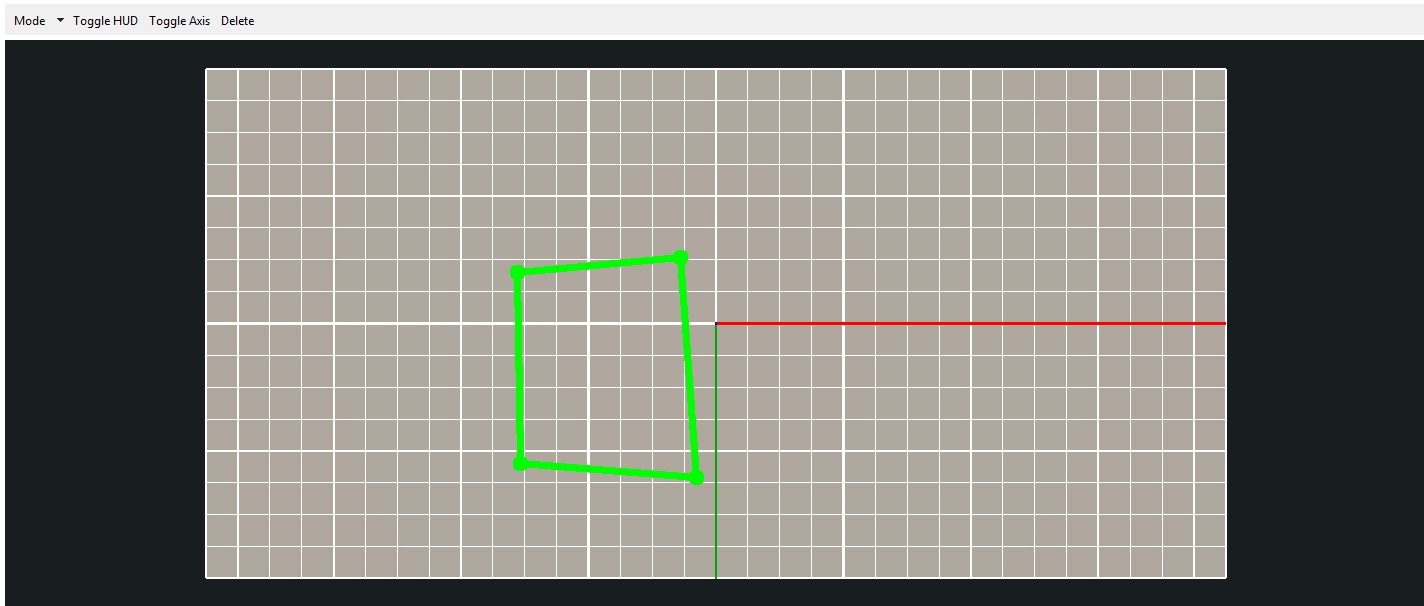
\includegraphics[width=12cm]{images/AddPolygon}
\centering
\caption{A new polygon, colored green because the user has not yet permanently
added it to the mesh.}
\label{fig:addpolygon}
\end{figure}

Click again to make the polygon permanent, signified by turning purple, or hit
\texttt{Esc} to cancel.

\begin{figure}[!h]
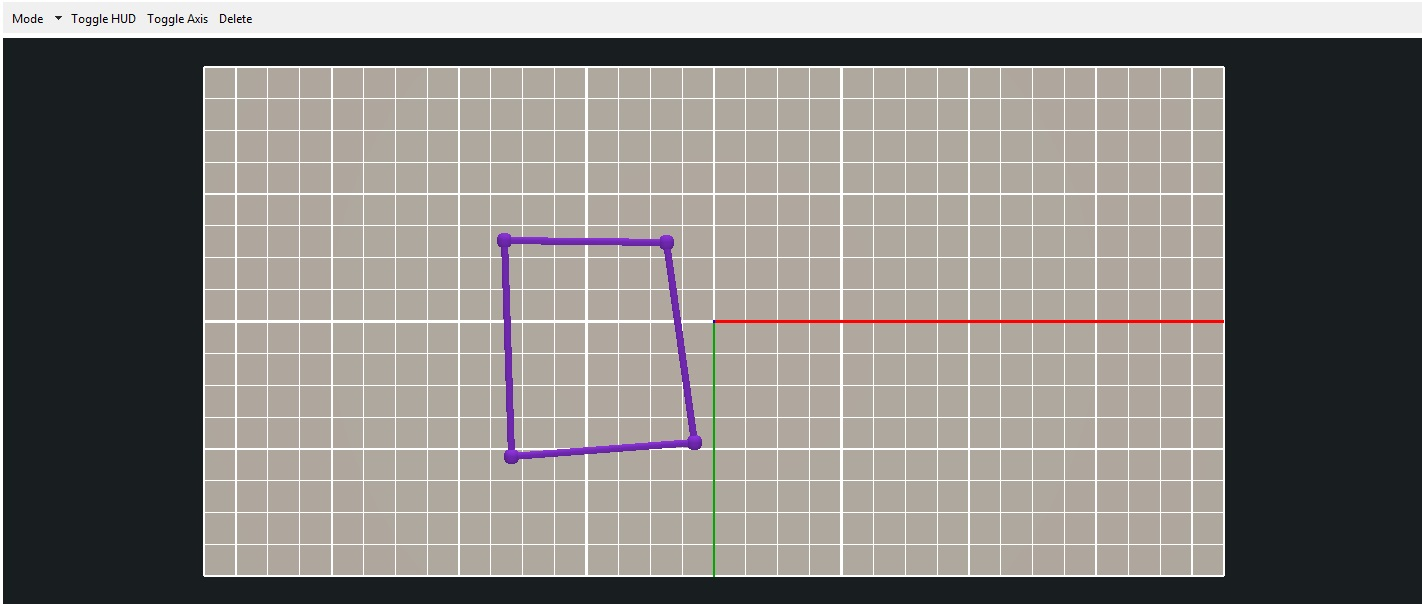
\includegraphics[width=12cm]{images/NewPolygon}
\centering
\caption{The polygon turns purple after clicking, showing that it has been
finished.}
\label{fig:newpolygon}
\end{figure}

The \texttt{Mode} button in the top left allows you to switch between
\texttt{Add Elements} mode, used previously, and \texttt{Edit Elements} mode.

\begin{figure}[!h]
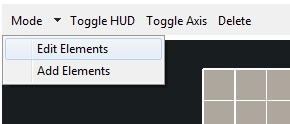
\includegraphics[width=12cm]{images/EditMode}
\centering
\caption{The \texttt{Mode} button allows switching between \texttt{Edit
Elements} mode and \texttt{Add Elements} mode.}
\label{fig:editmode}
\end{figure}

In edit mode, you can click a vertex (or vertices) to select them. 

\begin{figure}[!h]
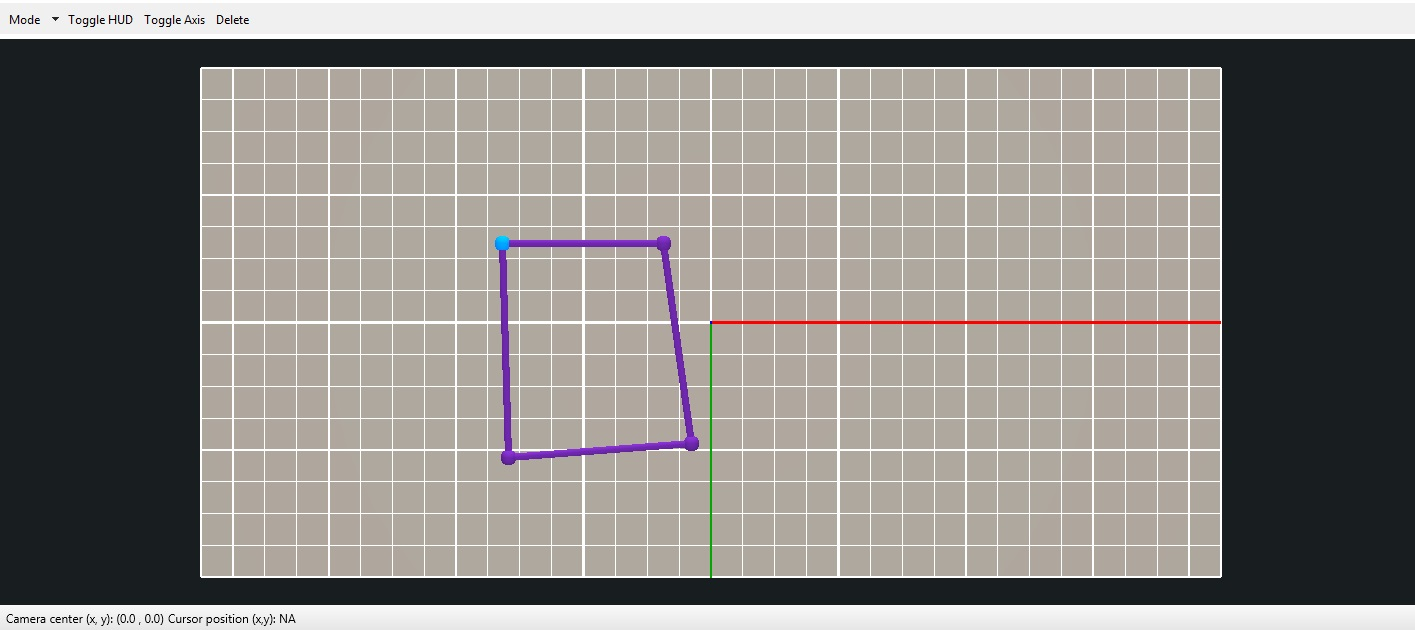
\includegraphics[width=12cm]{images/SelectedVertex}
\centering
\caption{A selected vertex will turn blue.}
\label{fig:selectedvertex}
\end{figure}

You can click and drag a vertex to move all selected vertices around the grid.

\section{Further Reading}

This tutorial has only given a brief overview of the ways in which you can use
ICE's visualization tools. For more detailed information, look under the
\texttt{docs} folder in the ICE repository. The visualization folder contains a
tutorial on the CSV and VisIt plots, while the geometryEditor and meshEditor
folders have tutorials on the geometry and mesh editors, respectively. 